\documentclass[landscape]{article}
\usepackage[landscape,margin=0.7in]{geometry}
\usepackage{pgfplots}
\usepackage{tikz}
\pgfplotsset{compat=1.18}

\begin{document}
\pagestyle{empty}

\begin{figure}
    \centering
    \begin{tikzpicture}
        \begin{axis}[
            title={\Large Back-to-Front Strategy - Zone 1 (Rows 16-19)},
            xlabel={Seat Column},
            ylabel={Row Number},
            xticklabels={A,B,C,D,E,F},
            ytick={1,2,3,4,5,6,7,8,9,10,11,12,13,14,15,16,17,18,19},
            xtick={0,1,2,3,4,5},
            xmin=-0.5,
            xmax=5.5,
            ymin=0.5,
            ymax=19.5,
            y dir=reverse,
            enlargelimits=false,
            axis on top,
            width=0.9\textwidth,
            height=0.4\textheight,
            colorbar,
            colormap={boarding}{
                color(0)=(white);
                color(0.5)=(yellow);
                color(1)=(purple)
            },
            colorbar style={
                title={Status},
                ytick={0,0.5,1},
                yticklabels={Empty,Boarding,Seated},
            },
            point meta min=0,
            point meta max=1
        ]
            
        % Initialize with back-to-front pattern (Zone 1 boarding - 16-19)
        \addplot[matrix plot, mesh/cols=6, point meta=explicit] table [meta=C] {
            x y C
            0 1 0
            1 1 0
            2 1 0
            3 1 0
            4 1 0
            5 1 0
            0 2 0
            1 2 0
            2 2 0
            3 2 0
            4 2 0
            5 2 0
            0 3 0
            1 3 0
            2 3 0
            3 3 0
            4 3 0
            5 3 0
            0 4 0
            1 4 0
            2 4 0
            3 4 0
            4 4 0
            5 4 0
            0 5 0
            1 5 0
            2 5 0
            3 5 0
            4 5 0
            5 5 0
            0 6 0
            1 6 0
            2 6 0
            3 6 0
            4 6 0
            5 6 0
            0 7 0
            1 7 0
            2 7 0
            3 7 0
            4 7 0
            5 7 0
            0 8 0
            1 8 0
            2 8 0
            3 8 0
            4 8 0
            5 8 0
            0 9 0
            1 9 0
            2 9 0
            3 9 0
            4 9 0
            5 9 0
            0 10 0
            1 10 0
            2 10 0
            3 10 0
            4 10 0
            5 10 0
            0 11 0
            1 11 0
            2 11 0
            3 11 0
            4 11 0
            5 11 0
            0 12 0
            1 12 0
            2 12 0
            3 12 0
            4 12 0
            5 12 0
            0 13 0
            1 13 0
            2 13 0
            3 13 0
            4 13 0
            5 13 0
            0 14 0
            1 14 0
            2 14 0
            3 14 0
            4 14 0
            5 14 0
            0 15 0
            1 15 0
            2 15 0
            3 15 0
            4 15 0
            5 15 0
            0 16 0.5
            1 16 1
            2 16 0.5
            3 16 0.5
            4 16 1
            5 16 0.5
            0 17 1
            1 17 1
            2 17 1
            3 17 1
            4 17 1
            5 17 1
            0 18 1
            1 18 1
            2 18 1
            3 18 1
            4 18 1
            5 18 1
            0 19 1
            1 19 1
            2 19 1
            3 19 1
            4 19 1
            5 19 1
        };
        
        % Draw aisle line
        \draw[black, thick, dashed] (axis cs:2.5,0.5) -- (axis cs:2.5,19.5);
        
        % Draw zone boundaries
        \fill[blue!20, opacity=0.3] (axis cs:-0.5,15.5) rectangle (axis cs:5.5,19.5);
        
        % Zone labels
        \node[right] at (axis cs:5.5,17.5) {Zone 1 (Current)};
        \node[right] at (axis cs:5.5,14) {Zone 2};
        \node[right] at (axis cs:5.5,11) {Zone 3};
        \node[right] at (axis cs:5.5,8) {Zone 4};
        \node[right] at (axis cs:5.5,5) {Zone 5};
        \node[right] at (axis cs:5.5,2) {Zone 6};
        
        % Time indicator
        \node[font=\Large] at (axis cs:2.5,20.5) {t = 3 minutes};
        
        % Description
        \node[draw, align=left, anchor=south west] at (axis cs:-0.5,-2) {
            \textbf{Back-to-Front Boarding Strategy:}\\
            • Aircraft divided into 6 zones from back to front\\
            • Passengers board in sequence: Zone 1 → Zone 2 → Zone 3 → Zone 4 → Zone 5 → Zone 6\\
            • Currently boarding: Zone 1 (Rows 16-19)\\
            • Reduced interference from previously seated passengers\\
            • Estimated total boarding time: 11.2 minutes
        };
        \end{axis}
    \end{tikzpicture}
\end{figure}

\begin{figure}
    \centering
    \begin{tikzpicture}
        \begin{axis}[
            title={\Large Back-to-Front Strategy - Zone 3 (Rows 10-13)},
            xlabel={Seat Column},
            ylabel={Row Number},
            xticklabels={A,B,C,D,E,F},
            ytick={1,2,3,4,5,6,7,8,9,10,11,12,13,14,15,16,17,18,19},
            xtick={0,1,2,3,4,5},
            xmin=-0.5,
            xmax=5.5,
            ymin=0.5,
            ymax=19.5,
            y dir=reverse,
            enlargelimits=false,
            axis on top,
            width=0.9\textwidth,
            height=0.4\textheight,
            colorbar,
            colormap={boarding}{
                color(0)=(white);
                color(0.5)=(yellow);
                color(1)=(purple)
            },
            colorbar style={
                title={Status},
                ytick={0,0.5,1},
                yticklabels={Empty,Boarding,Seated},
            },
            point meta min=0,
            point meta max=1
        ]
            
        % Initialize with back-to-front pattern (Zone 3 boarding - 10-13)
        \addplot[matrix plot, mesh/cols=6, point meta=explicit] table [meta=C] {
            x y C
            0 1 0
            1 1 0
            2 1 0
            3 1 0
            4 1 0
            5 1 0
            0 2 0
            1 2 0
            2 2 0
            3 2 0
            4 2 0
            5 2 0
            0 3 0
            1 3 0
            2 3 0
            3 3 0
            4 3 0
            5 3 0
            0 4 0
            1 4 0
            2 4 0
            3 4 0
            4 4 0
            5 4 0
            0 5 0
            1 5 0
            2 5 0
            3 5 0
            4 5 0
            5 5 0
            0 6 0
            1 6 0
            2 6 0
            3 6 0
            4 6 0
            5 6 0
            0 7 0
            1 7 0
            2 7 0
            3 7 0
            4 7 0
            5 7 0
            0 8 0
            1 8 0
            2 8 0
            3 8 0
            4 8 0
            5 8 0
            0 9 0
            1 9 0
            2 9 0
            3 9 0
            4 9 0
            5 9 0
            0 10 0.5
            1 10 0.5
            2 10 1
            3 10 1
            4 10 0.5
            5 10 0.5
            0 11 1
            1 11 1
            2 11 1
            3 11 1
            4 11 1
            5 11 1
            0 12 1
            1 12 1
            2 12 1
            3 12 1
            4 12 1
            5 12 1
            0 13 1
            1 13 1
            2 13 1
            3 13 1
            4 13 1
            5 13 1
            0 14 1
            1 14 1
            2 14 1
            3 14 1
            4 14 1
            5 14 1
            0 15 1
            1 15 1
            2 15 1
            3 15 1
            4 15 1
            5 15 1
            0 16 1
            1 16 1
            2 16 1
            3 16 1
            4 16 1
            5 16 1
            0 17 1
            1 17 1
            2 17 1
            3 17 1
            4 17 1
            5 17 1
            0 18 1
            1 18 1
            2 18 1
            3 18 1
            4 18 1
            5 18 1
            0 19 1
            1 19 1
            2 19 1
            3 19 1
            4 19 1
            5 19 1
        };
        
        % Draw aisle line
        \draw[black, thick, dashed] (axis cs:2.5,0.5) -- (axis cs:2.5,19.5);
        
        % Draw zone boundaries and highlight current zone
        \fill[blue!20, opacity=0.3] (axis cs:-0.5,9.5) rectangle (axis cs:5.5,13.5);
        
        % Zone labels
        \node[right] at (axis cs:5.5,17.5) {Zone 1 (Complete)};
        \node[right] at (axis cs:5.5,14) {Zone 2 (Complete)};
        \node[right] at (axis cs:5.5,11) {Zone 3 (Current)};
        \node[right] at (axis cs:5.5,8) {Zone 4};
        \node[right] at (axis cs:5.5,5) {Zone 5};
        \node[right] at (axis cs:5.5,2) {Zone 6};
        
        % Time indicator
        \node[font=\Large] at (axis cs:2.5,20.5) {t = 9 minutes};
        
        % Description
        \node[draw, align=left, anchor=south west] at (axis cs:-0.5,-2) {
            \textbf{Back-to-Front Boarding Strategy:}\\
            • Aircraft divided into 6 zones from back to front\\
            • Passengers board in sequence: Zone 1 → Zone 2 → Zone 3 → Zone 4 → Zone 5 → Zone 6\\
            • Currently boarding: Zone 3 (Rows 10-13)\\
            • Zones 1 and 2 already seated\\
            • Estimated total boarding time: 11.2 minutes
        };
        \end{axis}
    \end{tikzpicture}
\end{figure}

\end{document}